\subsection{Markers advection}\label{sec:runge}
The 2nd-order Runge-Kutta advection scheme in space is tested by means of the Zalesak disk test \citep{Zalesak1979,Thieulot2014}. The benchmark is performed
in a unit square domain with a grid resolution of $32\times32$ elements and 1000000 markers and values of Courant number between 0.25 and 1.
At $t=0$, the disk is centred at position $(0.5;0.75)$ with a radius $R=0.15$ and has a vertical fissure 0.05 wide and 0.2 high (orange in Fig. \ref{fig:runge})
and with the velocity field prescribed in the entire domain as
\begin{eqnarray}
u(x,y)&=&2\pi\left(y-\frac{L_x}{2}\right)\nonumber \\
v(x,y)&=&-2\pi\left(x-\frac{L_x}{2}\right)\nonumber
\end{eqnarray}
the markers are back to their initial location after a $2\pi$ rotation ($t=1$). The clockwise rotation of the disk at $t=0.25$, 0.5 and 0.75 
is shown in Fig. \ref{fig:runge} (red, blue and green, respectively). The distance from the centre of 1 marker is calculated throughout the rotation to
evaluate the error for different values of Courant number. As expected, the error increase with the increasing of the time step, as shown in 
Fig. \ref{fig:runge_err}. 
All data can be found at \url{https://github.com/aleregorda/Benchmarks/tree/main/Advection/Zalesak_Disk}.

\begin{figure}
\centering
\includegraphics[width=200px]{./Figures/Zalesak.pdf}
\caption{Position of the Zalesak disk at $t=0$, 0.25, 0.5 and 0.75 (orange, red, blue and green, respectively) for the case with Courant number of 1.}
\label{fig:runge}
\end{figure}

\begin{figure}
\centering
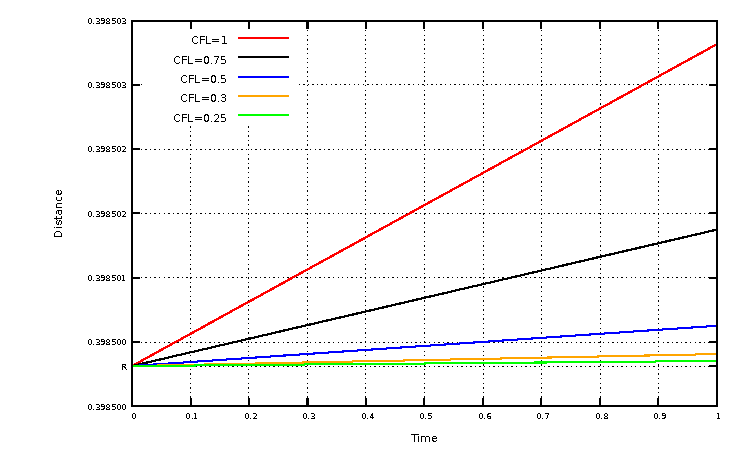
\includegraphics[width=400px]{./Figures/zal_marker.pdf}
\caption{Distance from the centre as function of time for values of Courant number of  of 0.25, 0.3, 0.5, 0.75 and 1 (green, orange, blue, black and red,
respectively). R indicates the distance from the centre considering a perfect circle trajectory.}
\label{fig:runge_err}
\end{figure}